\section{Coordinate descent methods}
In this section we describe the basic idea behind coordinate descent methods in general, and derive a serial coordinate descent deconvolution algorithm. This algorithm replaces CLEAN in the Major/Minor cycle architecture. The algorithm we describe here is serial in the sense that each step of the algorithm has to finish before the next step can be started. Each individual step can use multiple processors, as we show with a GPU-accelerated implementation. Later in Section \ref{pcdm} we will introduce more sophisticated parallel coordinate descent methods.

We call the coordinate descent algorithm "basic", because it can be seen as a special case of more complicated coordinate descent methods\cite{richtarik2016distributed, richtarik2016parallel}, which we will discuss later in Section. Here, we derive efficient CPU- and GPU- implementation and show how we can use MPI for a naive distributed deconvolution algorithm.



\subsection{Elastic net regularization} \label{cd:reg}
\begin{figure}[h]
	\centering
	\begin{subfigure}[b]{0.3\linewidth}
		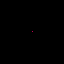
\includegraphics[width=\linewidth]{./chapters/03.distribution/L1.png}
		\caption{Effect of the pure L1 norm ($\lambda$ = 1.0) on a single point source.}
		\label{cd:elastic:L1}
	\end{subfigure}
	\begin{subfigure}[b]{0.3\linewidth}
		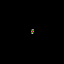
\includegraphics[width=\linewidth]{./chapters/03.distribution/L2.png}
		\caption{Effect of the pure L2 norm ($\lambda$ = 1.0) on a single point source.}
		\label{cd:elastic:L2}
	\end{subfigure}
	
	\caption{Effect of the L1 and L2 Norm separately.}
	\label{cd:elastic}
\end{figure}

This regularization is a mixture between the L1 and L2 regularization. The Figure \ref{cd:elastic} shows the effect of the L1 and L2 norm on a single star. The L1 regularization forces the image to contain few non-zero pixels as possible. It encodes our prior knowledge that the image will contain stars. The L2 regularization on the other hand "spreads" the single star across multiple pixels. This forces the image to represent extended emissions, like hydrogen cloud, with a large number of non-zero pixels (the L1 norm tends to break extended emissions apart, only using a handful of non-zero pixels). The L2 norm was already used in other image reconstruction algorithms in radio astronomy\cite{ferrari2014distributed}, with the downside that the resulting image will not be sparse.

Elastic net mixes these two norms together, becoming "sparsifying L2 norm". It retains the sparsifying property of the L1 norm, while also keeping extended emissions in the image. Formally, elastic net regularization is defined as the following:

\begin{equation}\label{cd:elastic:formula}
ElasticNet(x, \alpha) = \: \alpha \left \|x \right \|_1 + \frac{1-\alpha}{2}  \left \|x \right \|_2
\end{equation}

Elastic net has three properties which make it an interesting regularization for coordinate descent: It was shown to speed up convergence rates compared to the pure L1 or L2 norm\cite{friedman2010regularization}, is a separable function, and has a closed form solution. The first property was not further investigated in this work. The second property, separability, means that we can calculate the regularization for each pixel independently of each other, and we still arrive at the same result. Lastly, we can find a simple formula for each pixel that applies the elastic net regularization:

\begin{equation}\label{cd:elastic:closed}
ElasticNetClosedForm(x, \lambda ,\alpha) = \: \frac{max(x - \lambda * \alpha, 0)}{1+\lambda(1 - \alpha)}
\end{equation}

The closed form solution \eqref{cd:elastic:closed} of the elastic net regularization is also a mixture of the closed form solutions of the L1 and L2 norm. The closed form solution of the L1 norm is shrinkage: $max(x - \lambda, 0)$, we reduce the pixel value by $\lambda$ and clamp negative values. For the L2 norm, we divide the pixel value: $\frac{x}{1+\lambda}$.

%Proximal operator But the second property leads to an optimization algorithm 

Note that the shrink operation in this project always clamps negative pixels to zero. We constrain the image to only contain zero or positive pixel values. This has become a widely used constraint in radio interferometric image reconstruction and may lead to improved image quality\cite{mcewen2011compressed}.

Elastic net is the regularization we use throughout this work. It is separable (we can calculate it for each pixel independently) and has an easy to compute closed form solution.

\subsection{Serial coordinate descent}
Why it is serial.